\chapter{Evaluation}
\label{ch:evaluation}
% terminology: attentional data = 'focus rate'
[not yet complete]

This chapter presents results of number of experiments we have run. This includes 
We report on the feedback that is received from users' interaction through the use of the wePorter web interface. We show how it can be used for the purposes of filtering segments of interest within a video and the configuration of a new video story from the initially unstructured content. We present results from a user evaluation study on the merit of filtered and reconfigured content. We end with a reflection on our results in the discussion section.




\section{Preliminary Experiments}
\label{sec:preliminary_experiments}

\subsection{Positional Bias}
Positioning two video's one on top of the other, might inflict a bias for users in their attentional behaviour. It might be the case that videos on the top are systematically more attended to than videos displayed below. We've experimented to see whether such positioning bias effects occur.

To see whether the positioning of a video has effect on users' attentional behaviour, we've presented two groups of users the same two videos playing in parallel and varied their relative positioning. In two trials, participants were divided by random into control group and test group. The first trial was conducted with 37 participants (24 control, 13 test), the second with 32 (18 control, 14 test). In each trial, test group participants were show the same two videos as the control group, but their positioning was flipped. Figure \ref{fig:exp_posbias} shows a visual explanation of the experimental setup.

\begin{figure}[htbp]
  \centering
    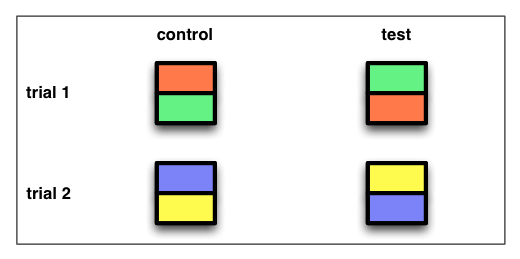
\includegraphics[width = .7\textwidth]{img/exp_posbias}
  \caption{Setup for Positional Bias Experiment}
  \label{fig:exp_posbias}
\end{figure}


\subsection{Context Dependency}
We propose a statistical analysis of interaction data to inform the reconfiguration of initially unstructured video parts. We hypothesise that:
\begin{enumerate}
  % \item The perceived quality of a video reconfiguration is dependent on the sequential ordering of its internal parts
  \item Users' attentional behaviour depends on the sequential ordering of video parts
  \item Data about users' attentional behaviour can indicate what are preferred orderings.
\end{enumerate}

Before we investigate the second hypothesis in section \ref{sec:main_experiments}, we must scrutinise the first. In order to test whether users' attentional behaviour is dependent on the sequential ordering of video parts we have run a experiment in two trials. The first of these had 35 participants, the second 28. In each trial participants were presented with with a two sequences of three video parts playing back continuously using the parallel video player described in section \ref{sec:weporter_interface}. Based on random picks, roughly half of the participants were labelled as control group the others as test group. Participants in this group where shown two sequences where all video parts originated from different sources. This was changed for the second group, where participant were shown parts across the sequences that clearly belong to the same source video. 

The first trial presented test group users with a first part in the bottom sequence that was followed by a part from the same source video as the third part in the top video. The second trial presented test group users with pieces from the same source video in the first and third part of the top sequence and second part of the bottom sequence. The baseline sequences shown to control group participants had video parts of different sources on all positions and had final parts of both sequences identical to test group users. A visual description of these conditions is shown in figure \ref{fig:exp_context}. Where we use the same conventions to display sequences, video parts and colouring to indicate source videos as in figure \ref{fig:framework}.

\begin{figure}[htbp]
  \centering
    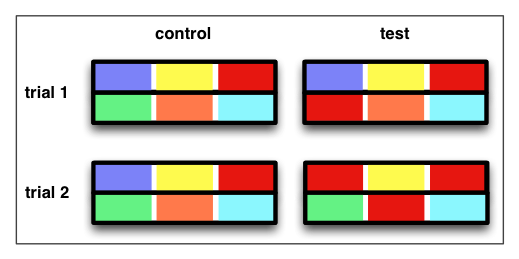
\includegraphics[width = .7\textwidth]{img/exp_context}
  \caption{Setup for Context Dependency Experiment}
  \label{fig:exp_context}
\end{figure}





\section{Main Experiments} % (fold)
\label{sec:main_experiments}

Our main experiments use the system framework described in section \ref{sec:weporter_implementation} for the preparation and presentation of video content, data capture from user interaction and storage of interaction data. The experiments we report on here are based on the interactions from a total of 68 persons over a period of a week.

\section{Setup}
For our main experiments we use a set of 10 unedited, user-generated videos that were returned in response to a query for ``Diamond Jubilee London'' on YouTube. The videos along with their title, length and current view count is shown in table \ref{videos}. As mentioned in section \ref{sec:weporter_implementation}, we divide source videos into video parts of equal length and generate two sequences consisting of an equal number of video parts to present in parallel. In our main experiments 

% TODO Table
\begin{table}
   % \begin{tabular}{ | l | l | p{8cm} | p{1.3cm} | l |}
   \begin{tabular}{ | l | l | p{8cm} | p{1.3cm} | l |}
     \hline
     \textbf{Id} & \textbf{File Name}	          & \textbf{Title}	  & \textbf{Length (sec)} & \textbf{Views} \\ \hline
     1	 & ``jubilee\_01.webm''	& ``Diamond Jubilee London 5th June 2012 The Mall Video 3'' & 186                             & 45   \\ \hline
     2	 & ``jubilee\_02.webm''	& ``Diamond jubilee London 5th June 2012 The Mall'' & 47                                      & 108  \\ \hline
     3	 & ``jubilee\_03.webm''	& ``London Thames - Queens Diamond Jubilee Pageant - Dunkirk Little Ships, June 2012'' & 234  & 2304\\ \hline
     4	 & ``jubilee\_04.webm''	& ``My Diamond Jubilee video!'' & 54                                                          & 28   \\ \hline
     5	 & ``jubilee\_05.webm''	& ``Queens Barge. Diamond Jubilee London 2012 VIDEO Ursula Maxwell-Lewis 0053'' & 163         & 88   \\ \hline
     6	 & ``jubilee\_06.webm''	& ``Queens diamond jubilee London 5th June 2012'' & 30                                        & 43   \\ \hline
     7	 & ``jubilee\_07.webm''	& ``Queens Diamond Jubilee Procession, 5th June 2012, London, UK'' & 133                      & 58   \\ \hline
     8	 & ``jubilee\_08.webm''	& ``Queens Elizabeth 60th Diamond Jubilee London 2012. 1st'' & 73                             & 203  \\ \hline
     9	 & ``jubilee\_09.webm''	& ``Queens Elizabeth 60th Diamond Jubilee London 2012. 2nd'' & 165                            & 246  \\ \hline
     10 & ``jubilee\_11.webm''	& ``Queens Elizabeth 60th Diamond Jubilee London 2012. 14th'' & 390                           & 88   \\ \hline
   \end{tabular}
   \caption{Source Videos used for the main experiments (Views count accessed on 23-09-2012)}
   \label{videos}
\end{table}

% if all views were parallel plays
The videos used for the main experiments have a total length of 25 minutes and their individual view counts range from 28 to 2304. 


\subsection{Clean Data} % (fold)
\label{sub:clean_data}

Data returned from the capturing of attentional behaviour in the parallel player interface might have several deficiencies that we account for by preprocessing the data before we start analysis. These range from inaccurate artifacts induced by the interface to users' behaviour patterns that make their data less revealing.


% subsection clean_data (end)

\subsection{Landscapes of Attention} % (fold)
\label{sub:landscapes_of_attention}

The distinction to be made, between interesting intervals on one hand and less striking parts of a video on the other is not likely to be a very strict one. After all, an unedited video captures a single stretch of space and time, so any event that is of particular interest will unlikely have hard cut-off points in time. Rather, if we see interest as a function of time in a particular video, we would expect a somewhat continuous flowing line with spikes every now and then when an interesting event occurs. 

Looking at interest at a more global level, aggregating over a large group of users, would result in an even a more smooth landscape of interest. This kind of data reveals mountains and valleys that can be used for attention-based segmentation. From the thus segmented parts, the ones with high attentional scores can be returned as candidates for interesting parts within a video.

% subsection landscapes_of_attention (end)

\subsection{Evaluating Focus} % (fold)
\label{sub:evaluating_focus}

By capturing the amount of focus time, we receive measures for user attention. We hope these measures for attention help point to patterns in user preference. If the two dimensions turn out to be linked, it makes sense to base segmentation of potentially interesting parts of video on the focus data captured in our parallel play interface.

To see how focus measures relate to user preference, we compare video parts which have received low focus rates

% subsection evaluating_focus (end)


% section main_experiments (end)

\section{Questionnaire} % (fold)
\label{sec:questionnaire}

% section questionnaire (end)

\section{Discussion} % (fold)
\label{sec:discussion}

This section presents a discussion of the results presented in this chapter as well as considerations about wePorter at system level. We also relate the findings from our experimentation with the wePorter system back to the broader ideas concerned Human Computation towards meaningful video analysis.

\subsection{Potential Extensions} % (fold)
\label{sub:potential_in_real_context}
% at YT viewed a lot
Using the length of individual videos and the number of times they have been viewed, we have calculated that the total time spent on watching the 10 videos above, amounts to over 185 hours. That is a lot of user interaction that could help in the computation of the most interesting video segments. If directed through our one minute parallel play interface, all this user interaction would result in more than 11000 complete interactions. With 12 video parts presented in each interaction, it would amount to more than 130000 attentional ratings for video parts or over 900 ratings per part. 

% filtering can be applied
This is not yet regarding the system's filtering functionality. Once reliable estimates of user interest have been established from the collection of captured attentional ratings, we can filter for the parts that seem most interesting, that way enabling a convergence towards the most interesting video segments. A simple way of doing this would be to rank all video parts according to their average attentional rating and discard the parts that are systematically less attended to, on the assumption that they are considered less interesting. More complex procedures are of course possible, for example taking into account the number of ratings a part has received, the positions in sequence at which parts have been presented or the kind of users that have submitted the interactions (e.g. first time users versus experienced users). Once the initial set of source videos has been filtered, more data can be acquired for the remaining set, after which filtering can be applied again. This iterative process of filtering can continue until the process yields a small subset of video part that have acquired most attention in aggregate.

% if filtering applied
Filtering video parts to converge to a subset of the source videos that is  iteratively narrowed down, means that most interactive computation will be focussed on the video parts that receive most attention. There is an obvious issue of exploration versus exploitation here. When is filtering applied and what part of the current set of content is discarded in an iteration.

% subsection potential_in_real_context (end)

\subsection{Feedback from Comments} % (fold)
\label{sub:feedback_from_comments}

\begin{quote}
  ``[...]the technology may though have many uses like the crowd sourcing of video editing or the training of AI to mimic human audio visual focus and attention'' - Mia
\end{quote}

As part of the user feedback form that was presented during the experiments, participants were given the option to leave their comments. Thinking of the potential of the interface, some comments, like the one above, hit the nail right on the head. Others touched upon different aspects of the experiment, the interface and the content of the videos. Overall a number of salient points emerged from the comments:

\begin{itemize}
  \item \textbf{``I would like to see news this way''} - People were positive about the way video was presented in parallel and were enthusiastic about the possibility to interact.
  \item \textbf{``I believe there was a bug''} - A number of people reported difficulties in the playback of videos. Most issues concerned one or more video parts not immediately playing after the preceding one had finished. Besides causing data to be less clean, this caused some users to be confused.
  \item \textbf{``The subject and content of the videos was uninteresting''} - Many people said they were not particularly interested in the topic of the presented videos. This meant that often they weren't drawn strongly to a particular video and did not feel a strong reason to shift focus from one or another.
\end{itemize}

Some participants also offered ideas as to how they saw the project could be extended:

\begin{quote}
  ``Idea is great and project full of potential, in particular for big events which are well covered and allow multi-angle views of an action. It would be interesting to have information about the content producer displayed discretely on the player. That way the audience could vote on the quality of a source, and in time reward the owner for it's content, encouraging him to submit more videos in this system.'' - Marc
\end{quote}

% subsection feedback_from_comments (end)

% section discussion (end)





